% Este archivo es parte de la memoria del proyecto fin de carrera
% de Aarón Bueno Villares. Protegida bajo la licencia GFDL.
%
% Para más información, la licencia completa viene incluida en el
% fichero fdl-1.3.tex

% Copyright (C) 2010 Aarón Bueno Villares

\section{Historial de desarollo}
\label{sec:desarrollo}

En ésta sección se contarán todas las vivencias acaecidas durante el
desarrollo del proyecto, hasta su estado actual, y un poquito de
cuáles serán los siguientes pasos a dar.

Las versiones publicadas de la aplicación son las versiones desde la
v0.1, v0.2, v0.3, v0.5 y v0.7. A partir de la versión 3, no he tomado
ninguna captura de pantalla, pero puedes ver los videos de cada
versión en youtube, con solo buscar \fpt.

\subsection{En busca de un motor gráfico}
Al comenzar el desarrollo, tuve claro que deseaba hacer algo similar,
en apariencia, a \textit{gource}, pero quizás debido a comentarios
externos, no quise usar openGL pues creía que sería una biblioteca
demasiado difícil de usar. Comencé usando el motor 3D de
\textit{Ogre}, y tras una semana de aprendizaje y agonía, intentando
dibujar primitivas, acabé abandonándo \textit{Ogre} y decidí entrar de
lleno en openGL.

En éste estado, tenía un rudimentario diseño y una simple clase árbol,
que usaba para hacer pruebas. El proyecto, o al menos el día en que
inicialicé el repositorio (creo que inicialicé el repositorio el mismo
día en que comencé a programar) fué el 23 de Octubre del 2010. El 12
de Noviembre ya hice mi primer \textit{commit} en \textit{openGL}. Éste traslado
fue sencillo ya que usé \textit{gource} para aprender a programar en
\textit{openGL}, y éste usaba SDL como gestor de ventanas, librería
que ya conocía. Para imprimir en \textit{gource}, hice uso de
funciones muy básicas para las que no hace falta tener mucha
experiencia, y al día siguiente ya dibujaba un árbol con iluminación
en los nodos, usando los gráficos de gource. La captura que subí al
blog (véase al final) el mismo día fué la siguiente:

\begin{center}
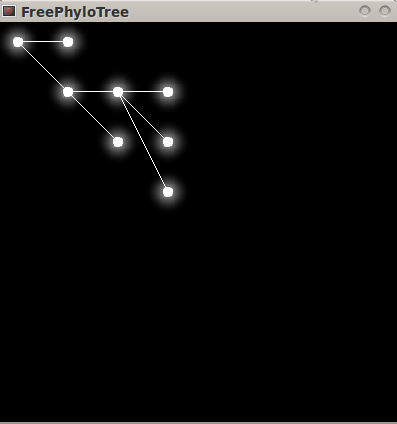
\includegraphics[scale=.65]{images/arbolBlur.png}
\end{center}

\subsection{En busca de un algoritmo de visualización de grafos}
Como vemos en la imágen anterior, los nodos se imprimían con un
primitivo algoritmo de posicionado de nodos. Sencillamente, los hijos
de un nodo se desplazaban a la izquierda unos 50 puntos, y cada
hermano unos 40 puntos en dirección vertical. Los nietos se solapaban
siempre entre sí, y la captura del ejemplo está diseñada para que ésto
no ocurriese.

Estaba claro que me hacía falta un algoritmo de visualización de
grafos, y ésto era una tarea algo más dura. Empecé a documentarme
sobre algoritmos de visualización de árboles, pero ninguna me
convencía, primero, porque no eran algoritmos animables: la posición
de cada nodo se calculaba en un solo paso, y además, los árboles se
imprímian de modo que los hijos se dibujasen, respecto a sus padres,
siguiendo siempre una misma dirección. En la imágen adjuntada arriba, por
ejemplo, los hijos se van imprimiendo en dirección
derecha-izquierda. Yo, repito una vez más, quería visualizar el árbol
tal y como lo hace gource, donde la raíz está en el centro del árbol
con sus hijos a su alrededor, y además, de forma animada.

Lo que hace gource, en realidad, es usar un algoritmo de visualización
general de grafos para visualizar el árbol. Éstos algoritmos siempre
son iterativos, y para conseguir la animación, gource imprime cada uno
de éstos pasos. El algoritmo de visualización que usa gource para
imprimir el árbol es uno basado en quadtrees, y debido a que viendo el
código no comprendía como funcionaba el algoritmo, y buscando en
internet tampoco (además, no sabía que algoritmo concreto usaba
gource), decidí buscar algún documento general sobre visualización de
grafos.

Encontré la tesis doctoral de Andrés Aiello y Rodrigo Ignacio
Silveira, llamado \textbf{Trazado de grafos mediante métodos dirigidos
  por fuerzas: revisión del estado del arte y presentación de
  algoritmos para grafos donde los vértices son regiones
  geográficas}. En ésta tesis doctoral, como dice el título de la
tesis, hay un primer apartado de repaso histórico de los diversos
algoritmos, y el que implementé fué el primer algoritmo que la
historia de la visualización de grafos ha ofrecido: \textit{spring
  embedder}. En el blog (véase al final) hay una entrada completa que
explica en qué consiste dicho algoritmos.

El 27 de Diciembre ya tenía implementado el algoritmo, y sobre el día
30 tenía un algoritmo de coloreado, donde cada nodo se hace cargo de
una región del cubo cromático, y sus hijos van, a su vez,
repartiéndose dicha región, de modo que nodos más cercanos tengan
colores más similares. El 31 de Diciembre fué mi último commit con
SDL, y, en suma, me manejaba con la cámara y podía expandir y contraer
árboles, así como ampliar el radio de destello cuando los nodos se
expande, de forma similar a lo que hace gource. Todas éstas fueron las
características de la versión v0.2.

\subsection{En busca de un explorador integrado}
En la versión v0.2 tenía dos carencias importantes, primero, que
todavía no había explorador integrado y, segundo, que el árbol no se
construía automáticamente, sino que creada los nodos uno a uno desde
el propio código. El siguiente paso era, primero, conseguir el
explorador, para lo que ví la necesidad de usar Qt y desterrar SDL.

Nunca había usado Qt y no sabía como se programaba bajo dicha librería
pero, a decir verdad, la experiencia ha sido muy satisfactoria, puesto
que es muy completo y está muy bien documentado. Tiene un widget
openGL para que allí se renderizen todas las instrucciones openGL, y
también dispone de un widget para mostrar páginas web. Con éste
explorador, en el momento en que el usuario hacia doble click
izquierdo en un nodo, usaba el nombre del taxón para abrir la página
de wikipedia correspondiente, y funcionaba a la perfección sin mucho
esfuerzo. Ésto fué logrado el 14 de Enero del 2011, día en que
publiqué la versión v0.3 de la aplicación, subí un video a youtube y
actualicé el blog.

\subsection{En busca de un nuevo diseño}
\subsubsection{Rama 3D}
En todo éste tiempo, desde que comencé con openGL, he usado varias
fuente para aprender: el libro de openGL, el código de gource y la
inestimable ayuda de Pepe Cullera, al que conocí gracias a una
cuestión sobre el uso de primitivas en Ogre que dejé en el foro
español de Ubuntu, antes de pasarme a openGL. Desde entonces, Pepe me
ha ayudado en muchas ocasiones con openGL.

Tras ver la versión v0.2 del proyecto, le gustó la idea y decidió
desarrollar conmigo. El 15 de Enero se abrió una rama nueva llamada
3ddelopment en la que Pepe Cullera, que domina muy bien openGL,
desarrollara un árbol en 3D, lográndolo en unos 10 días de trabajo.

Debido a que el árbol en 3D, para árboles grandes, no ofrece una
visualización cómoda, y hasta que no se le saque una buena utilidad
(¿quizás para visualizar moléculas orgánicas o genes en un futuro \----muy
lejano por cierto?), no se fusionará con la rama de trabajo
principal.

\subsubsection{Nuevo diseño}
Por mi parte, cambié completamente el diseño de la aplicación,
experimenté con c++0x usando el mecanismo de \textit{variadic
  templates} para manejar una clase vector de un número indeterminado
de dimensiones, así como la directiva \textit{auto} para que el
compilador resuelva por tí el tipo, sin tener que escribirlo
manualmente \----ésto evita tener declaraciones de iteradores
inmensas\----. El mecanismo de plantillas múltiples acabé eliminándolo
debido a que hacía a la ejecución de la aplicación muy lenta. Este
«episodio» de trabajo finaliza el 12 de Marzo.

\begin{center}
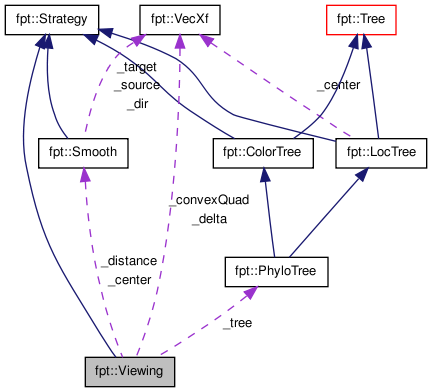
\includegraphics[scale=.65]{images/classDiagram.png}
\end{center}

En el cambio global del diseño, había dos cosas principales que quise
arreglar:
\begin{itemize}
\item La clase árbol tenía demasiada información de diversos aspectos
  que quería desacoplar: información de color, de posición, de ulr's
  de wikipedia, etcétera.
\item Había un comportamiento en común, en muchos puntos del código,
  que quería encapsular: muchos movimientos de la aplicación son
  suavizados, es decir, si un elemento ha de cambiar de posición, no
  cambia de forma brusca, sino suavizada, de modo que el elemento se
  dirige a su nueva posición mediante un parámetro $\delta$ que indica
  el porcentaje de actualización de la posición: un valor $\delta=0.5$
  significa que el elemento, en un solo paso, se mueve la mitad del
  espacio que queda hasta su destino, en su siguiente paso se moverá
  la mitad de lo que quede, y así sucesivamente hasta que esté lo
  suficientemente cerca para finalizar el movimiento. De éste
  comportamiento participan los movimientos de los nodos, sus colores, el
  explorador de wikipedia \----aunque para el explorador ya lo
  quité\----, la cámara, y posteriormente también el buscador que
  añadí y el menú de ayuda.
\end{itemize}

En la imágen adjunta arriba puede verse una parte del esquema del
diseño como ejemplo. La clase \textit{PhyloTree} ahora es la herencia
de un árbol de color y un árbol de posición, que son, a su vez,
árboles. La clase \textit{Viewing}, la responsable de
manejar la cámara, usa la clase \textit{Smooth}, que es la que se
encarga del suavizado de movimientos, ya que la cámara está
suavizada. A su vez, los nodos de color o de posición, que son los que
componen al árbol de color y al árbol de posición también tienen sus
atributos en forma de objetos suavizados.

\subsection{En busca de un cladograma automático}
La segunda gran asignatura pendiente era la construcción automática
del cladograma. Es la recta final de la construcción de la versión
v0.5.

¿Cómo lo conseguí? Pues en un día de intenso trabajo del 14 al 15 de
Marzo. Usé la librería \textit{libcurl}, librería que ya tenía
señalada desde hacía tiempo y ya tenía ciertas nociones de cómo
manejarla, terminé de aprender a usarla, a su vez que aprendía a hacer
consultas al API de MediaWiki. Tuve ciertos problemas con el contexto
de comunicación HTTP desde el software al API, pero con algunos
\textit{googleos} terminé de arreglarlos.

Al principio las consultas se realizaban también contra
\textit{wikipedia} dado que cada artículo tiene una ficha de taxón con
la información de los subclados.

Para hacer éstas consultas, cada taxón tiene en su artículo una
plantilla llamada \textbf{ficha de taxón}. Esta ficha esta siempre
localizada en el mismo lugar del artículo, así que es fácilmente
localizable en el texto. A su vez, los subclados están en un lugar muy
concreto de la ficha del taxón. Lo que no está tan claro es la forma
en que estos subclados son presentados, que varían mucho de taxón a
taxón.

En vista de los problemas que me ocasionaba, decidí construir el árbol
desde wikispecies, porque tengo varias ventajas: el lugar en el que se
encuentran los subclados de un clado dado es igual de claro que en el
caso de wikipedia, y además, la forma en que éstos subclados se
presentan varías mucho menos de taxón a taxón. Además, wikispecies es
más completo y contiene un número muchísimo mayor de taxones, lo que
hace al árbol más completo y al analizador más robusto.

Por último, cabe citar que, a la par que construía el árbol a partir
de wikispecies, también incluí flex como analizador léxico \----antes
buscaba y filtraba el texto a mano. Gracias a flex, ahora el análisis
es mucho más rápido y también es más cómodo extraer los clados. La
versión v0.5 se publicó, como anuncio de todos éstos cambios, el 15 de
Marzo.

\subsection{En busca de una aplicación más completa}
La aplicación tenía ya grandes progresos en funcionalidad, pero había
un campo en el que todavía era un poco pobre, que era la
interactuación con el usuario.

El usuario no sabe qué opciones ofrece el programa cuando lo ejecuta,
ni tampoco tiene opción de explorar directamente un taxón. Cuando se
ejecutaba la aplicación, se cargaba el clado neomura, un clado muy
alto en la jerarquía. Hacían falta más de 15 pasos para llegar al
taxón primates, y el usuario no podía llegar directamente. Ésto era
una carencia importante, y además un problema sabiendo que la fase
final del premio local de Cádiz estaba al caer (martes 22 de
Marzo). Así que añadí un buscador el sábado 20 de Marzo e hice muchos
cambios menores en el código, añadí un documento de README y otro de
INSTALL, actualicé la documentación (sólo las clases) y la página
principal.

Después del concurso, del que salí victorioso, seguí mejorando la
aplicación. Añadí un menú de ayuda donde se ven los controles posibles
de la aplicación, la posibilidad de podar ramas \----quedarte con un
subárbol\----, la posibilidad de fijar nombres de las especies a
voluntad \----antes sólo se visualizaban los nombres cuando ponías el
ratón encima de un nodo\---- y también hice mejoras en cuestión de
eficiencia y cámaras, así como hacer un analizador léxico más robusto,
ya que había taxones que el analizador no reconocía debido a que no
estaban resuelto todos las posibles formas de presentación de los
mismos. Todo ésto me valió una versión v0.7, que cree el 30 de Marzo,
y no publiqué en el blog hasta el día siguiente, día que en que
también hice el último \textit{commit}.

\subsection{En busca de un futuro}
No sé seguro cuál será el siguiente paso a dar, pero en
\textit{wikispecies} hablé de hacer ciertos cambios en la presentación
de los artículos de los taxones para uniformarlos más, y al final la conversación
finalizó por un camino paralelo,
discutiendo sobre algo que no era lo que originalmente proponia y no
ha vuelto a reabrirse, aunque con esa discusión comprendí que sí, que
yo debería tener mi propia wiki.

Luego envíe un correo al blog \textit{la ciencia y sus demonios}
anunciando \fpt, pero no me han contestado todavía. Luego descubrí que
la web \textit{palaeos} había trasladado su página a un wiki, y ese
wiki es lo que más se parece a lo que mi aplicación desea ofrecer, así
que en cuanto tenga tiempo, me pondré en contacto con ellos.
